\documentclass[10pt,letterpaper]{article}

\usepackage[margin=0.75in]{geometry}
\usepackage{tikz}
\usepackage{graphicx}
\usepackage{amsmath}
\graphicspath{{img/}}
\begin{document}

  \title{Stats 314, Data Analysis \#3}
  \author{Cody Malick\\
  \texttt{malickc@oregonstate.edu}}
  \date{\today}
  \maketitle

\section*{Part I}
\subsection*{Scenario 1}
C. One sample t test\\
We want to use a one sample t test because we know the population average of 38
hours. Because we know the population average, we can compare the sample mean
with the population mean to make a decision as to whether or not the sample mean
if better or worse than the population mean.

\subsection*{Scenario 2}
D. Matched pairs t test
We have two sets of sample means, before and after, and we want to determine if
there was an improvement or not. This is perfect for a matched pair t test.

\subsection*{Scenario 3}
B. Two sample t test
The two sample t test is used to see if two sets of averages are equal, or if
one is better than the other. 

\subsection*{Scenario 4}
A. One sample z test for a mean
Given the information we have, we can see that the sample mean is relatively
close to the population mean, with a low standard deviation. This is usually
indictive of a normal distribution. But we want to use this test to see if a
given null hypothesis holds or is rejected. In this case, the null hypothesis
would be weight = 77 lbs. 

\section*{Part II}
\subsection*{a}
$\mu = 69.63938$\\
$\sigma = 4.066723$\\
The population is 256\\
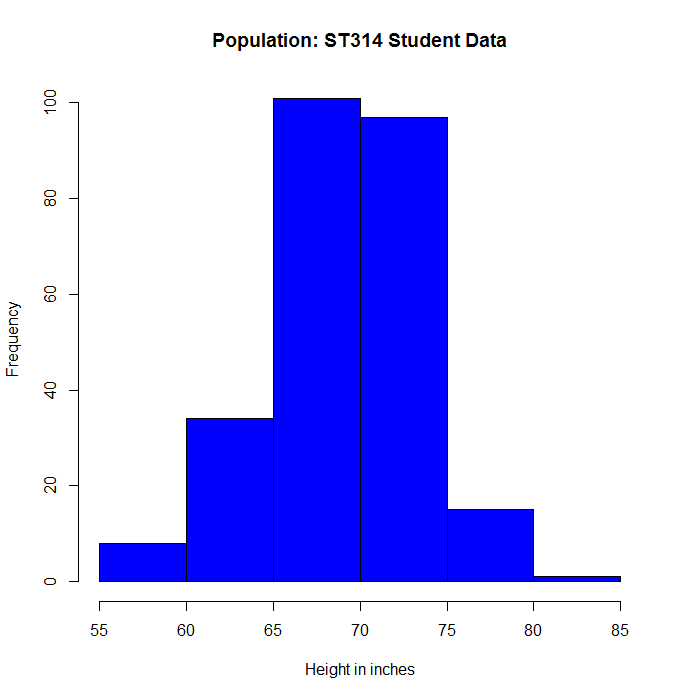
\includegraphics[scale=.5]{student-hist}\\
The majority of the population falls between 65 inches and 75 inches in height.
\subsection*{b}
$\bar{x}=69.88$\\
$s=5.325411$\\
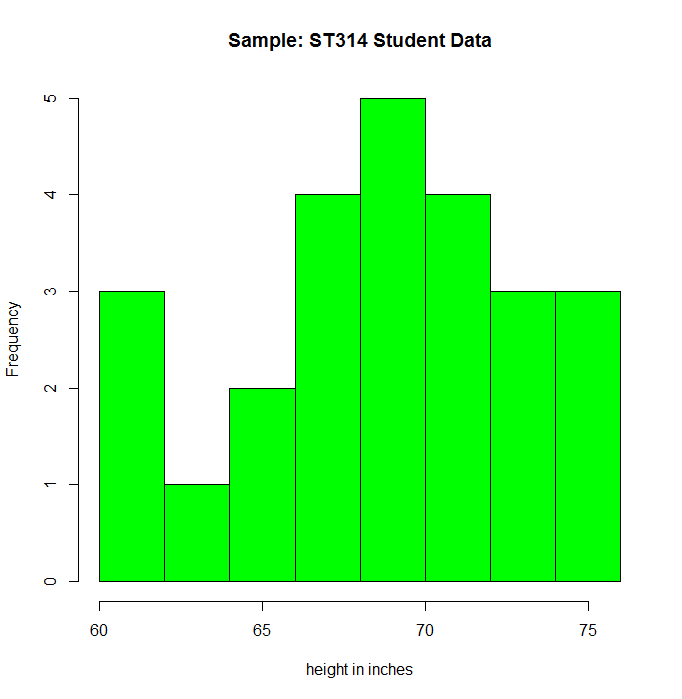
\includegraphics[scale=.5]{sample-student-hist}\\
The sample distribution isn't as radical as the population distribution was.
Most members of the sample lie in the 60-75 range, as our population sample 
did. The sample mean was almost exactly the same as the population mean, and
the sample standard deviation was a little bit higher.

\subsection*{c}
$CI=69.88 \pm 1.96*\frac{4.066723}{\sqrt{25}}\\
=71.47416$ and $=68.285844$\\
The $95\%$ confidence interval for the height of the class is estimated to be
between $68.2858$ and $71.4742$ inches, with a point estimate of $69.88$.
\subsection*{d}
To calculate the t confidence interval for mean height, we do use the following
formua:\\
$CI=\bar{x}\pm t^* * \frac{s}{\sqrt{n}}$\\
$69.88 \pm 2.064*\frac{5.3254}{\sqrt{25}}$\\
$=72.0783$ and $=67.6817$\\
The $95\%$ confidence interval for the height of the sample from class is
estimated to be between $67.6817$ and $72.0783$ inches, with a point estimate
of $69.88$.\\
This interval does include the true population mean of $69.6394$.\\

\subsection*{e}
The difference between parts c and d are that, in one, we're taking the CI of
the sample knowing what the population standard deviation is, while in part d,
we're taking the CI not known the population SD. The two answers we got are not
that different from each other.

\section*{Part III}
\subsection*{a}
I would anticipate that we would reject the null hypothesis as our sampled data
from our previous measurements had a slightly different mean. I suspect it's
enough to reject.
\subsection*{b}

\subsection*{c}


\section*{Part IV}
\subsection*{a}

\subsection*{b}

\subsection*{c}


\section*{Part V}
\subsection*{a}

\subsection*{b}

\subsection*{c}

\subsection*{d}

\subsection*{e}

\subsection*{f}

\subsection*{g}

\subsection*{h}

\subsection*{i}

\subsection*{j}

\end{document}
